\documentclass{article}
\usepackage[binary-units=true]{siunitx}
\usepackage{array}
\usepackage{graphicx}
\begin{document}

\title{Pagination 32-bit}
\author{jeremshy}
\maketitle

Upper portion of a virtual address is used to to identify a series of paging-structure entries.The last of these entries identifies the physical address of the region to which the linear address translates (called the \textbf{page frame}). The lower portion of the linear 	address (called the \textbf{page offset}) identifies the specific address within that region to which the linear address translates.\\

The first paging structure is located at the pysical address in CR3. \\
A page directory comprises 1024 32-bit entries (PDEs). For this reason, the translation process uses 10 bits at a time from a 32-bit linear address.\\
\\

\noindent
Bits 31:22 identify the first paging-structure entry. (Page directory)\\
Bits 21:12 identify a second. The latter identifies the page frame. (Page table)\\
Bits 11:0 of the linear address are the page offset within the 4-KByte page frame ($2^{12} = 4096$)\\

Si une page est mappe depuis la premiere etape (un seul niveau de referencement), alors la page frame fait $2^{22} = \SI{4194304}{\kibi\byte}$ = $\SI{4}{\mega\byte}$.

A directory is located at the physical address specified in bits 31:12 of CR3.\\

\begin{tabbing}
A PD contains 1024 PDE, a PDE is selected using the PA defined as follows :\\
\hspace{1cm}\=Bits 39:32 are all 0\\
\>Bits 31:12 are from CR3.\\
\>Bits 11:2 are bits 31:22 of the linear address.\\
\>Bits 1:0 are 0\\ 
\end{tabbing}

\flushleft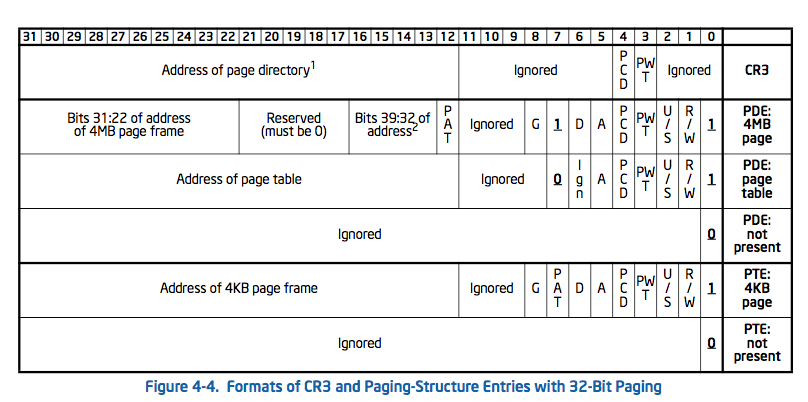
\includegraphics[scale=0.59]{cr3_graph.png}

\end{document}
